\documentclass[10pt,twocolumn]{article}

\usepackage[a4paper,margin=1cm]{geometry}
\usepackage[utf8]{inputenc}
\usepackage[T1]{fontenc}
\usepackage[brazil]{babel}
\usepackage{amsmath}
\DeclareUnicodeCharacter{00D7}{\ensuremath{\times}}
\DeclareUnicodeCharacter{2192}{\ensuremath{\to}}
\usepackage{listings}
\usepackage{xcolor}
\usepackage{booktabs}
\usepackage{graphicx}
\usepackage{titlesec}

% Titulos menores (orientacao recebida em aula)
\titleformat{\section}{\small\bfseries}{\thesection.}{0.4em}{}
\titlespacing*{\section}{0pt}{3pt}{1pt}
\setlength{\parskip}{0pt}
\setlength{\columnsep}{8pt}
\linespread{0.92}\selectfont

\lstset{
    basicstyle=\ttfamily\scriptsize,
    breaklines=true,
    numbers=left,
    numberstyle=\tiny,
    frame=single,
    language=C,
    keywordstyle=\color{blue},
    commentstyle=\color{gray}
}

% Gerado por benchmark/analise.py -- nao editar a mao.
\newcommand{\TabForte}{%
\begin{tabular}{@{}ccccccc@{}}
\toprule
Unidades & Tempo (s) & S & E (%) & CV (%) & Mcel/s & Init (s) \\
\midrule
4 & 10,938 & 5,3 & 133 & 0,0 & 110 & 0,407 \\
8 & 5,516 & 10,6 & 132 & 0,1 & 218 & 0,407 \\
16 & 2,874 & 20,3 & 127 & 0,9 & 418 & 0,421 \\
32 & 1,484 & 39,3 & 123 & 0,1 & 809 & 0,495 \\
64 & 1,461 & 39,9 & 62 & 1,0 & 821 & 0,654 \\
4×4 & 2,875 & 20,3 & 127 & 1,1 & 417 & 0,405 \\
4×8 & 2,905 & 20,1 & 63 & 0,1 & 413 & 0,408 \\
4×16 & 1,485 & 39,2 & 61 & 0,3 & 808 & 0,406 \\
\bottomrule
\end{tabular}}
\newcommand{\TabFraca}{%
\begin{tabular}{@{}ccccccc@{}}
\toprule
Unidades & Tempo (s) & S & E (%) & CV (%) & Mcel/s & Init (s) \\
\midrule
4 & 1,419 & 5,1 & 128 & 0,1 & 106 & 0,053 \\
8 & 1,425 & 10,2 & 128 & 0,2 & 210 & 0,106 \\
16 & 1,464 & 19,9 & 124 & 0,4 & 410 & 0,219 \\
32 & 1,485 & 39,3 & 123 & 0,1 & 808 & 0,422 \\
4×4 & 1,462 & 19,9 & 125 & 1,1 & 410 & 0,203 \\
4×8 & 2,905 & 20,1 & 63 & 0,0 & 413 & 0,409 \\
\bottomrule
\end{tabular}}
\newcommand{\TabHT}{%
\begin{tabular}{@{}cccccc@{}}
\toprule
Versão & 32 físicos (s) & S & 64 com HT (s) & S & Ganho (%) \\
\midrule
MPI puro (p = 32 → 64) & 1,484 & 39,3 & 1,461 & 39,9 & 2 \\
Híbrida (4×8 → 4×16 thr) & 2,905 & 20,1 & 1,485 & 39,2 & 96 \\
\bottomrule
\end{tabular}}


% Procura os fontes na propria pasta do main.tex, em src/ ou em ../src/.
\newcommand{\includecodigo}[1]{%
  \IfFileExists{#1}{%
    \lstinputlisting[language=C]{#1}%
  }{%
    \IfFileExists{src/#1}{%
      \lstinputlisting[language=C]{src/#1}%
    }{%
      \IfFileExists{../src/#1}{%
        \lstinputlisting[language=C]{../src/#1}%
      }{%
        \textbf{Arquivo \texttt{#1} não encontrado.}%
      }%
    }%
  }%
}

\title{\vspace{-1.5cm}\large Jogo da Vida de Conway com MPI no modelo fases
paralelas: versão pura e híbrida MPI/OpenMP\vspace{-0.3cm}}
\author{
    \normalsize
    Bruno Neves \quad
    Guilherme Hoffmann \quad
    João Sbardelotto \\
    \small Computação Paralela, Turma 320, Prof. Cesar A. F. De Rose,
    PUCRS, Grupo 12
}
\date{}

\begin{document}
\maketitle
\vspace{-1.0cm}

\section{Introdução}
\label{sec:intro}

Este trabalho implementa o \emph{Jogo da Vida de Conway} no modelo
\emph{fases paralelas} com MPI: cada processo
fica com $1/np$ do tabuleiro e um ciclo de geração avança por fases
(processamento local, verificação distribuída coletiva e troca com os
vizinhos), executadas simultaneamente por todos os processos. São
apresentadas uma versão \textbf{MPI puro} e uma \textbf{híbrida
MPI/OpenMP}, executadas na atlântica com 4 nós (32 núcleos físicos, 64 com
HT; na híbrida, 4 processos (um por nó) com 4, 8 e 16 threads).

\section{Modelagem no modelo fases paralelas}
\label{sec:modelo}

O tabuleiro é um toro de \emph{altura} $\times$ \emph{largura} células
(4000$\times$4000, 75 gerações, densidade inicial de 20\%,
\texttt{srand(42)}). A partição é por \textbf{blocos de linhas}: o processo
$r$ fica com as linhas $[r\cdot h/np,\,(r{+}1)\cdot h/np)$; cada processo
\textbf{gera internamente} a sua fatia percorrendo a mesma sequência de
\texttt{rand()} da versão sequencial e gravando só as suas linhas, com
tabuleiro inicial idêntico à linha de base, sem comunicação.

Cada geração é um ciclo de fases:
\begin{itemize}\setlength{\itemsep}{0pt}
  \item \textbf{Processamento local (Fase 1):} cada processo calcula a próxima
        geração das suas linhas, usando \emph{ghost rows}: a primeira e a
        última linha de cada fatia têm cópias das linhas de borda dos
        vizinhos, trocadas com \texttt{MPI\_Sendrecv} (duas chamadas, uma para
        cada sentido do toro vertical). Com o halo, o núcleo por célula é o
        mesmo da versão sequencial, só sem os módulos verticais.
  \item \textbf{Verificação distribuída (Fase 2, coletiva):} cada processo
        conta quantas células suas mudaram de estado e um
        \texttt{MPI\_Allreduce} soma o total. Se ninguém mudou, o tabuleiro
        estabilizou e o trabalho está pronto (a geração seguinte seria
        idêntica); caso contrário, a execução segue até o limite de gerações.
  \item \textbf{Troca com vizinhos (Fase 3):} nova troca de \emph{ghost rows}
        em busca de convergência (que é a Fase 1 do ciclo seguinte).
\end{itemize}

Na versão \textbf{híbrida}, a Fase 1 de cada processo é paralelizada com
OpenMP: as linhas da fatia são repartidas estaticamente entre as threads do
nó (custo por linha uniforme). A comunicação MPI fica fora da região
paralela (granularidade grossa, sem MPI aninhado): \emph{MPI divide os nós,
OpenMP divide os núcleos}.

\section{Metodologia}
\label{sec:metodo}

Compilação com \texttt{-O2}; medições com \texttt{MPI\_Wtime} (média de 5
repetições), em 4 nós exclusivos da atlântica (8 núcleos físicos por nó,
2 sockets de 4, 16 com HT):
\begin{itemize}\setlength{\itemsep}{0pt}
  \item sequencial (\texttt{-N 1 -n 1}) como linha de base;
  \item \textbf{MPI puro}: $np = 4, 8, 16, 32$ (físico) e $64$ (HT);
  \item \textbf{híbrida}: 4 processos (1 por nó) $\times$ 4, 8 e 16 threads
        por nó (16 com HT), pontos comparáveis a $np=16$, $32$ e $64$ do
        MPI puro.
\end{itemize}
Na híbrida, \texttt{srun --hint=nomultithread} ($t{\le}8$) ou
\texttt{multithread} ($t{=}16$) é essencial: sem ele, o
\texttt{--cpus-per-task=8} recebia só os 8 CPUs de um socket, ou seja, 4 dos 8
núcleos físicos (detalhe na Seção~\ref{sec:analise}). Correção conferida por
checksum FNV-1a do tabuleiro final, igual ao da versão sequencial para todas
as configurações (inclusive alturas não divisíveis e mais processos que
linhas). A instrumentação cronometra, por rank, as fases de cálculo, troca de
halo e coletiva, e também a geração da fatia inicial ($O$(tabuleiro), fora do
cronômetro principal).

\section{Resultados}
\label{sec:resultados}

O sequencial leva \emph{58,3~s} (20,6 Mcel/s). As Tabelas~\ref{tab:forte} e
\ref{tab:fraca} e as Figuras~\ref{fig:forte}, \ref{fig:fraca} e~\ref{fig:eficiencia} (página
seguinte) mostram escalabilidade forte, fraca e eficiência do MPI puro e da
híbrida; a Tabela~\ref{tab:ht} isola o efeito do HT. Destaques: $S = 39{,}3$
com 32 processos no MPI puro ($E = 123\%$, superlinear) e $S = 37{,}7$ na
híbrida $4{\times}8$; a comunicação é irrelevante em todas as configurações;
o tempo de inicialização chega a 45\% do total em $np=64$.

\section{Análise}
\label{sec:analise}

\textbf{Superlinearidade por cache.} O speed-up supera o linear ($E$ de
123--133\% até 32 unidades) nas duas escalas: o tabuleiro de 4000$^2$
(32~MB nos dois tabuleiros) não cabe na cache do nó quando o sequencial
percorre tudo em um núcleo, mas dividido em fatias de 0,5~MB por rank as
fatias ficam residentes. A coluna Mcel/s evidencia: 20,6 no sequencial
contra 809 com $np=32$ (39$\times$).

\textbf{A comunicação não é gargalo.} A Figura~\ref{fig:fases} decompõe o
tempo por rank: em $np=32$, cada rank gasta 1,43~s de cálculo contra
0,0105~s de troca de halo e 0,063~s de Allreduce (75 gerações), menos de
5\% do total. O CV do cálculo entre ranks fica $\le 1{,}2\%$: as fatias
(blocos de linhas com resto distribuído) balanceiam bem.

\textbf{HT agrega pouco.} Duplicar as unidades de 32 para 64 (Tabela
\ref{tab:ht}) adiciona apenas 1,5\% no MPI puro e 2,7\% na híbrida: o
cálculo é limitado por memória, e os irmãos de HT dividem os mesmos
recursos do núcleo físico.

\textbf{O custo de inicializar.} Cada processo gera sua fatia percorrendo
\emph{todo} o tabuleiro de \texttt{rand()} ($O$(tabuleiro)
independente de $np$, ~0,41~s). Com o tempo total caindo para 1,5~s, o
init vira 27--45\% da execução em $np \ge 32$ (e cresce com a contenção de
cache: 0,65~s em $np=64$).

\textbf{Diagnóstico e correção de um desvio de medição.} A primeira rodada
da híbrida mostrava $4{\times}8$ tão lenta quanto $4{\times}4$ ($S=20$
ambas; Figura~\ref{fig:anomalia}, barras ``antes''). Com
\texttt{srun --cpu-bind=verbose} e \texttt{OMP\_DISPLAY\_ENV=verbose}
identificamos a causa: a topologia dos nós é 2 sockets $\times$ 4 núcleos
com HT e o kernel numera os CPUs com os pares em um socket e os ímpares no
outro; o \texttt{--cpus-per-task=8} recebia exatamente os 8 CPUs de um
único socket (4 núcleos físicos, com o socket restante ocioso; calc
$= W/16$ em vez de $W/32$, com $W \approx 45{,}7$ core$\cdot$s). A correção
foi \texttt{--hint=nomultithread}, que entrega um CPU por núcleo físico nos
dois sockets: o calc do $4{\times}8$ caiu de 2,84 para 1,46~s e o speed-up
saltou de 20,1 para 37,7, empatando com o MPI puro de mesmo tamanho
($4{\times}16$ e $4{\times}4$ não mudaram, como esperado).

\section{Ferramentas de IA}
\label{sec:ia}

O código, o suíte de benchmark e a análise foram desenvolvidos com apoio de
assistente de IA (Claude/opencode): instrumentação das fases, scripts
\texttt{benchmark.py}/\texttt{analise.py}, diagnóstico do binding
(interpretação dos logs \texttt{--cpu-bind=verbose}) e confecção deste
relatório. Todas as decisões, revisões e validações no cluster foram do
grupo.

% =====================================================================
% PAGINA 2: TABELAS E GRAFICOS (coluna simples)
% =====================================================================
\clearpage
\onecolumn

\section*{Tabelas e gráficos}
\vspace{-4pt}
\noindent\small 4 nós exclusivos da atlântica (2 sockets $\times$ 4 núcleos
por nó, 16 CPUs lógicas, HT). Tabuleiro 4000$\times$4000, 75 gerações,
densidade 20\%. $T_s = 58{,}3$~s (sequencial); na fraca, tabuleiro de
$125$ linhas por unidade e $T_s$ medido no tabuleiro grande de cada ponto.
Unidade = 1 processo MPI (pura) ou 1 thread OpenMP (híbrida, $4{\times}t$);
``64'' usa HT. Mcel/s = milhões de célula$\cdot$gerações por segundo;
CV = coeficiente de variação do cálculo entre ranks; Init = maior tempo de
geração da fatia entre os ranks.

\begin{table}[h]
\centering
\small\textbf{Escalabilidade forte (tabuleiro fixo)}\\[2pt]
\scriptsize\TabForte
\caption{MPI puro e híbrida, tabuleiro 4000$\times$4000.}
\label{tab:forte}
\end{table}

\begin{table}[h]
\centering
\small\textbf{Escalabilidade fraca (tabuleiro proporcional, sem HT)}\\[2pt]
\scriptsize\TabFraca
\caption{Tabuleiro de 125 linhas por unidade.}
\label{tab:fraca}
\end{table}

\begin{table}[h]
\centering
\small\textbf{Efeito do hyperthreading (forte)}\\[2pt]
\scriptsize\TabHT
\caption{32 unidades físicas $\times$ 64 com HT.}
\label{tab:ht}
\end{table}

\begin{figure}[h]
\centering
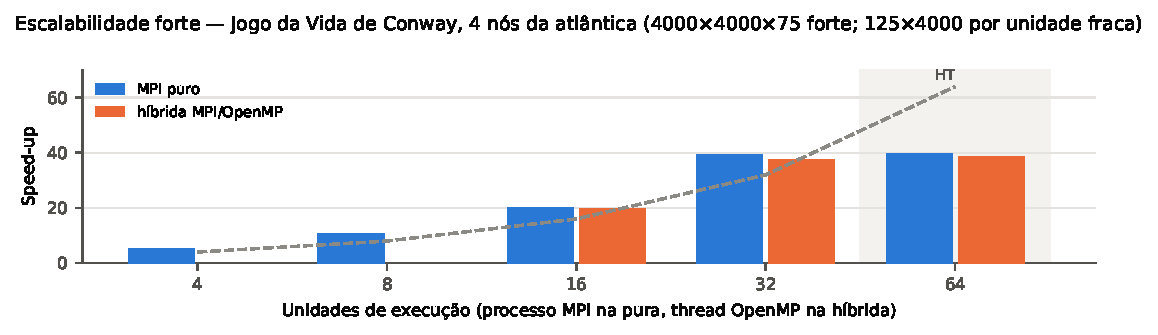
\includegraphics[width=0.72\linewidth]{fig_forte.pdf}
\caption{Escalabilidade forte: MPI puro (azul) e híbrida (laranja); ideal
$S=p$ tracejado, HT sombreado.}
\label{fig:forte}
\end{figure}

\begin{figure}[h]
\centering
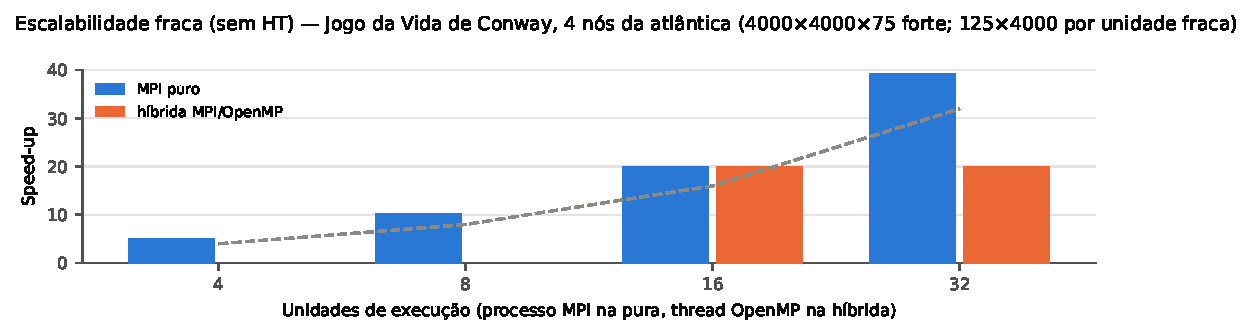
\includegraphics[width=0.72\linewidth]{fig_fraca.pdf}
\caption{Escalabilidade fraca (sem HT).}
\label{fig:fraca}
\end{figure}

\begin{figure}[h]
\centering
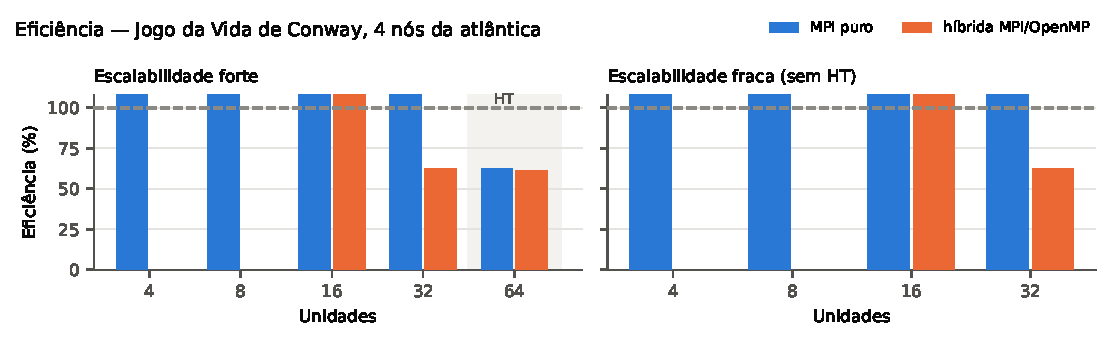
\includegraphics[width=0.85\linewidth]{fig_eficiencia.pdf}
\caption{Eficiência nas escalas forte e fraca.}
\label{fig:eficiencia}
\end{figure}

\begin{figure}[h]
\centering
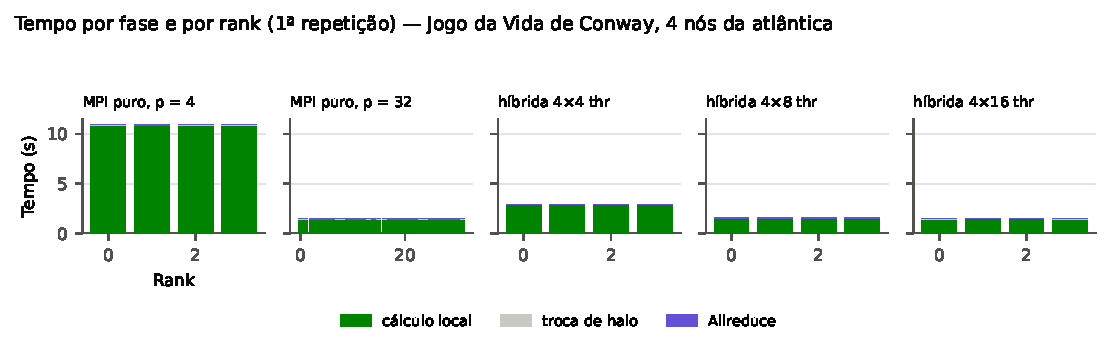
\includegraphics[width=0.85\linewidth]{fig_fases.pdf}
\caption{Tempo por fase e por rank (1ª repetição): o cálculo domina e a
comunicação (halo + Allreduce) é marginal.}
\label{fig:fases}
\end{figure}

\begin{figure}[h]
\centering
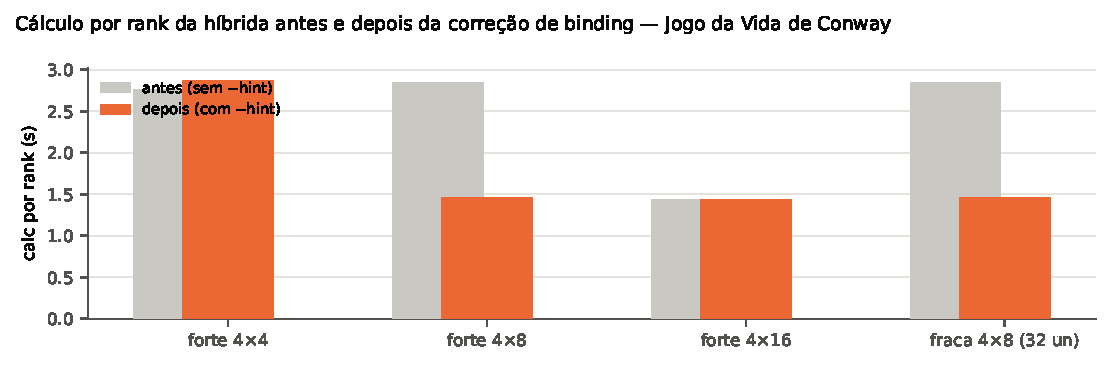
\includegraphics[width=0.72\linewidth]{fig_anomalia.pdf}
\caption{Cálculo por rank da híbrida antes e depois da correção de binding:
sem o \texttt{--hint}, o \texttt{--cpus-per-task=8} recebia só os CPUs de um
socket (4 dos 8 núcleos físicos).}
\label{fig:anomalia}
\end{figure}

\onecolumn
\appendix

\section{Versão sequencial (conwaySequencial.c)}
\includecodigo{conwaySequencial.c}

\section{Versão MPI puro (conway\_fases\_mpi.c)}
\includecodigo{conway_fases_mpi.c}

\section{Versão híbrida MPI/OpenMP (conway\_fases\_mpi\_omp.c)}
\includecodigo{conway_fases_mpi_omp.c}

\end{document}
